% !TeX root = main.tex
\chapter{Collaborative Manipulation}\label{ch:collaborative}
Our objective in this chapter is developing an adaptive control for a collaborative task of manipulating a large object with unknown parameters. As the task involves convergence and circulation of the object along a predefined curve, we use the control strategy developed in \cref{ch:vector_field} as a reference for velocity tracking. Our final control system can be thought of as a two-stage controller: the first one is kinematic and outputs the necessary velocity to guarantee curve tracking; the second controller is a dynamic one, responsible for ensuring that the object's velocity is equal to the kinematic controller output. We begin by presenting the system modelling, then we move to the vector field guidance employed in the kinematic controller, and finally, we present the adaptive control strategy.
\section{Modelling and problem statement} \label{sec:dynamic-modelling}
\begin{figure}[ht]
    \centering
    \def\svgwidth{.8\linewidth}
    \import{figures/}{collaborative_scheme.pdf_tex}
    \caption{Collaborative task}
    \label{fig:problem}
\end{figure}
The problem addressed in this section revolves around designing a controller to guide a manipulated object along a predefined curve $\mathcal{C} \subset \mathbb{R}^3\times \text{SO}(3)$\footnote{We adopt $\mathbb{R}^3 \times \text{SO}(3)$ here, though \citet{Muller2016} discusses the differences between this group and $\text{SE}(3)$ for dynamics, 
concluding $\text{SE}(3)$ is more appropriate.}. The object's dynamics include uncertain parameters like mass and geometric properties. With $N$ agents involved in the manipulation process, a decentralized control law is devised for each agent. The agents are unaware of their precise positioning relative to a measurement point. It is assumed that each agent possesses the capability to measure the pose and velocity of the object's measurement point.

We consider the cooperative manipulation of a rigid body by a team of $N$ autonomous agents, as illustrated in \cref{fig:problem}. The body undergoes both translations and rotations. We establish two reference frames: the world-fixed inertial frame denoted $\mathfrak{I}$, and the body-fixed frame denoted $\mathfrak{B}$, centered at the body's center of mass, $\mathbf{b}\triangleq\mathbf{b}^\mathfrak{I}$. Additionally, a body-fixed measurement point, $\mathbf{p}^\mathfrak{B}$, is situated at a distance $\mathbf{r}_p^\mathfrak{B}$ from the body's center of mass.

The body possesses a mass $m$ and a constant inertia tensor $\mathbb{I}_\text{cm}^\mathfrak{B}$ about its center of mass. We assume each agent is rigidly attached to the body at $\mathbf{r}_i$ from $\mathbf{p}^\mathfrak{B}$. While $\mathbf{r}_i$ ideally should be expressed relative to a frame at $\mathbf{p}^\mathfrak{B}$, for simplicity, we interchangeably consider $\mathbf{r}_i= \mathbf{r}_i^\mathfrak{B}$. This assumption is made under the understanding that this information solely pertains to torque computations, and the frame associated with the measurement point shares the same orientation as that of the center of mass. Each agent exerts a wrench $\boldsymbol{\tau}_i$ onto the body.


Let $\mathbf{p}\triangleq\mathbf{p}^\mathfrak{I}(t)$ be the position of the measurement point in $\mathfrak{I}$ and let $\mathbf{R}\triangleq \mathbf{R}_\mathfrak{B}^\mathfrak{I}(t)$ be the rotation matrix from frame $\mathfrak{B}$ to frame $\mathfrak{I}$. Let the linear velocity of the point $\mathbf{p}$ expressed in frame $\mathfrak{I}$ be represented by $\dot{\mathbf{p}}$, and let $\boldsymbol{\omega}\triangleq\boldsymbol{\omega}^\mathfrak{I}(t)$ denote the angular velocity of frame $\mathfrak{B}$ with respect to $\mathfrak{I}$, expressed in $\mathfrak{I}$. Additionally, let $\ddot{\mathbf{p}}$ and $\dot{\boldsymbol{\omega}}$ represent the linear and angular accelerations of the body, respectively. Then, we can express the linear velocity at $\mathbf{p}$ as
\begin{align}
    \dot{\mathbf{p}} &= \frac{d}{dt}\bigl(\mathbf{b} + \mathbf{R}\mathbf{r}^\mathfrak{B}_p\bigr) 
    = \dot{\mathbf{b}} +\SL[\boldsymbol{\omega}]\mathbf{R}\mathbf{r}^\mathfrak{B}_p + \mathbf{R}\dot{\mathbf{r}}^\mathfrak{B}_p = \dot{\mathbf{b}} +\SL[\boldsymbol{\omega}]\mathbf{R}\mathbf{r}^\mathfrak{B}_p,
\end{align}
where the fact that $\mathbf{r}^\mathfrak{B}_p$ is constant in frame $\mathfrak{B}$ was used. The linear acceleration is given by
\begin{align}
    \ddot{\mathbf{p}} &= \frac{d}{dt}\bigl(\dot{\mathbf{b}} +\SL[\boldsymbol{\omega}]\mathbf{R}\mathbf{r}^\mathfrak{B}_p\bigr) 
    = \ddot{\mathbf{b}} + \SL[\dot{\boldsymbol{\omega}}]\mathbf{R}\mathbf{r}^\mathfrak{B}_p + \SL[\boldsymbol{\omega}]\SL[\boldsymbol{\omega}]\mathbf{R}\mathbf{r}^\mathfrak{B}_p.
\end{align}
Thus, the resulting force acting on the body is given by Newton's second law as
\begin{align}
    \mathbf{F}^\mathfrak{I}&=m\ddot{\mathbf{b}} = m\bigl(\ddot{\mathbf{p}} - \SL[\dot{\boldsymbol{\omega}}]\mathbf{R}\mathbf{r}^\mathfrak{B}_p - \SL[\boldsymbol{\omega}]\SL[\boldsymbol{\omega}]\mathbf{R}\mathbf{r}^\mathfrak{B}_p\bigr).
\end{align}
The total torque at point $\mathbf{p}$ expressed in the inertial frame is given by
\begin{align}
    \mathbf{T}^\mathfrak{I}_p = \mathbf{R}\mathbf{T}^\mathfrak{B}_p = \mathbf{R}\mathbb{I}^\mathfrak{B}_\text{cm}\mathbf{R}^\top\dot{\boldsymbol{\omega}} + \SL[\boldsymbol{\omega}]\mathbf{R}\mathbb{I}^\mathfrak{B}_\text{cm}\mathbf{R}^\top\boldsymbol{\omega} - \SL[\mathbf{R}\mathbf{r}^\mathfrak{B}_p]\mathbf{F}^\mathfrak{I}, \label{eq:torque-modelling}
\end{align}
expanding the last term, we have
\begin{align}
    - \SL[\mathbf{R}\mathbf{r}^\mathfrak{B}_p]\mathbf{F}^\mathfrak{I} = 
    - \SL[\mathbf{R}\mathbf{r}^\mathfrak{B}_p]\ddot{\mathbf{p}} - \SL[\mathbf{R}\mathbf{r}^\mathfrak{B}_p]\SL[\mathbf{R}\mathbf{r}_p^\mathfrak{B}]\dot{\boldsymbol{\omega}} + \SL[\mathbf{R}\mathbf{r}^\mathfrak{B}_p]\SL[\boldsymbol{\omega}]\SL[\boldsymbol{\omega}]\mathbf{R}\mathbf{r}_p^\mathfrak{B}. \label{eq:partial-torque1}
\end{align}
From Steiner's theorem \citep{lemos2018analytical}, we know that $\mathbb{I}^\mathfrak{B}_p = \mathbb{I}^\mathfrak{B}_\text{cm} - m\SL[\mathbf{r}_p^\mathfrak{B}]^2$, where $\mathbb{I}^\mathfrak{B}_p$ is the inertia tensor about point $\mathbf{p}$. Thus, we can obtain the following expression for the second term in \eqref{eq:partial-torque1}
\begin{align}
    - \SL[\mathbf{R}\mathbf{r}^\mathfrak{B}_p]\SL[\mathbf{R}\mathbf{r}_p^\mathfrak{B}]\dot{\boldsymbol{\omega}} = - \mathbf{R}\SL[\mathbf{r}^\mathfrak{B}_p]\mathbf{R}^\top\mathbf{R}\SL[\mathbf{r}_p^\mathfrak{B}]\mathbf{R}^\top\dot{\boldsymbol{\omega}} = \mathbf{R}\bigl(\mathbb{I}^\mathfrak{B}_p - \mathbb{I}^\mathfrak{B}_\text{cm}\bigr)\mathbf{R}^\top\dot{\boldsymbol{\omega}}.
    \label{eq:partial-torque2}
\end{align}
Expanding the last term in \eqref{eq:partial-torque1}, we have
\begin{align}
    \begin{split}
        \SL[\mathbf{R}\mathbf{r}^\mathfrak{B}_p]\SL[\boldsymbol{\omega}]\SL[\boldsymbol{\omega}]\mathbf{R}\mathbf{r}_p^\mathfrak{B} &= \SL[\mathbf{R}\mathbf{r}^\mathfrak{B}_p]\SL[\boldsymbol{\omega}](\dot{\mathbf{p}} - \dot{\mathbf{b}})\\
        &= \SL[\mathbf{R}\mathbf{r}^\mathfrak{B}_p]\SL[\boldsymbol{\omega}]\dot{\mathbf{p}} - \SL[\mathbf{R}\mathbf{r}^\mathfrak{B}_p]\SL[\boldsymbol{\omega}]\dot{\mathbf{b}}.
    \end{split}
\end{align}
Applying Jacobi's identity, we obtain
\begin{align}
    % \begin{split}
    &m\SL[\SL[\dot{\mathbf{p}}]\mathbf{R}\mathbf{r}_p^\mathfrak{B}]\boldsymbol{\omega} + m\SL[\SL[\mathbf{R}\mathbf{r}_p^\mathfrak{B}]\boldsymbol{\omega}]\dot{\mathbf{p}}
    -m\SL[\SL[\dot{\mathbf{b}}]\mathbf{R}\mathbf{r}_p^\mathfrak{B}]\boldsymbol{\omega}  -m\SL[\SL[\mathbf{R}\mathbf{r}_p^\mathfrak{B}]\boldsymbol{\omega}]\dot{\mathbf{b}}\nonumber\\
    % &=-m\SL[\SL[\mathbf{R}\mathbf{r}_p^\mathfrak{B}]\dot{\mathbf{p}}]\boldsymbol{\omega}  -m\SL[\SL[\boldsymbol{\omega}]\mathbf{R}\mathbf{r}_p^\mathfrak{B}]\dot{\mathbf{p}}
    % -m\SL[\SL[\dot{\mathbf{b}}]\mathbf{R}\mathbf{r}_p^\mathfrak{B}]\boldsymbol{\omega}  +m\SL[\SL[\boldsymbol{\omega}]\mathbf{R}\mathbf{r}_p^\mathfrak{B}]\dot{\mathbf{b}}\nonumber\\
    &=-m\SL[\SL[\mathbf{R}\mathbf{r}_p^\mathfrak{B}]\dot{\mathbf{p}}]\boldsymbol{\omega}
    -m\SL[\dot{\mathbf{p}} - \dot{\mathbf{b}}]\dot{\mathbf{p}}
    -m\SL[\SL[\dot{\mathbf{b}}]\mathbf{R}\mathbf{r}_p^\mathfrak{B}]\boldsymbol{\omega}
    +m\SL[\dot{\mathbf{p}} - \dot{\mathbf{b}}]\dot{\mathbf{b}}\nonumber\\
    &=-m\SL[\SL[\mathbf{R}\mathbf{r}_p^\mathfrak{B}]\dot{\mathbf{p}}]\boldsymbol{\omega}
    +m\SL[\dot{\mathbf{b}}]\dot{\mathbf{p}}
    -m\SL[\SL[\dot{\mathbf{b}}]\mathbf{R}\mathbf{r}_p^\mathfrak{B}]\boldsymbol{\omega}
    +m\SL[\dot{\mathbf{p}}]\dot{\mathbf{b}}\nonumber\\
    &=-m\SL[\SL[\mathbf{R}\mathbf{r}_p^\mathfrak{B}]\dot{\mathbf{p}}]\boldsymbol{\omega}
    -m\SL[\SL[\dot{\mathbf{p}}-\SL[\boldsymbol{\omega}]\mathbf{R}\mathbf{r}_p^\mathfrak{B}]\mathbf{R}\mathbf{r}_p^\mathfrak{B}]\boldsymbol{\omega}\nonumber\\
    % &=-m\SL[\SL[\mathbf{R}\mathbf{r}_p^\mathfrak{B}]\dot{\mathbf{p}}]\boldsymbol{\omega}
    % -m\SL[\SL[\dot{\mathbf{p}}]\mathbf{R}\mathbf{r}_p^\mathfrak{B}]\boldsymbol{\omega}
    % + m\SL[\SL[\SL[\boldsymbol{\omega}]\mathbf{R}\mathbf{r}_p^\mathfrak{B}]\mathbf{R}\mathbf{r}_p^\mathfrak{B}]\boldsymbol{\omega}\nonumber\\
    &=-m\SL[\SL[\mathbf{R}\mathbf{r}_p^\mathfrak{B}]\dot{\mathbf{p}}]\boldsymbol{\omega}
    -m\SL[\boldsymbol{\omega}]\SL[\mathbf{R}\mathbf{r}_p^\mathfrak{B}]\dot{\mathbf{p}}
    - m\SL[\boldsymbol{\omega}]\SL[\mathbf{R}\mathbf{r}_p^\mathfrak{B}]\SL[\mathbf{R}\mathbf{r}_p^\mathfrak{B}]\boldsymbol{\omega}\nonumber\\
    &=-m\SL[\SL[\mathbf{R}\mathbf{r}_p^\mathfrak{B}]\dot{\mathbf{p}}]\boldsymbol{\omega}
    -m\SL[\boldsymbol{\omega}]\SL[\mathbf{R}\mathbf{r}_p^\mathfrak{B}]\dot{\mathbf{p}}
    - m\SL[\boldsymbol{\omega}]\mathbf{R}\bigl(\mathbb{I}^\mathfrak{B}_p-\mathbb{I}^\mathfrak{B}_\text{cm}\bigr)\mathbf{R}^\top\boldsymbol{\omega}. \label{eq:partial-torque3}
    % \end{split}
\end{align}
Finally, using \eqref{eq:torque-modelling}, \eqref{eq:partial-torque1}, \eqref{eq:partial-torque2}, and \eqref{eq:partial-torque3}, the resulting torque is expressed as
\begin{align}
    \begin{split}
        \mathbf{T}^\mathfrak{I}_p = &\mathbf{R}\mathbb{I}^\mathfrak{B}_\text{cm}\mathbf{R}^\top\dot{\boldsymbol{\omega}} + \SL[\boldsymbol{\omega}]\mathbf{R}\mathbb{I}^\mathfrak{B}_\text{cm}\mathbf{R}^\top\boldsymbol{\omega} - \SL[\mathbf{R}\mathbf{r}^\mathfrak{B}_p]\ddot{\mathbf{p}} + \mathbf{R}\bigl(\mathbb{I}^\mathfrak{B}_p - \mathbb{I}^\mathfrak{B}_\text{cm}\bigr)\mathbf{R}^\top\dot{\boldsymbol{\omega}} \\
        &-m\SL[\SL[\mathbf{R}\mathbf{r}_p^\mathfrak{B}]\dot{\mathbf{p}}]\boldsymbol{\omega}
        -m\SL[\boldsymbol{\omega}]\SL[\mathbf{R}\mathbf{r}_p^\mathfrak{B}]\dot{\mathbf{p}}
        - m\SL[\boldsymbol{\omega}]\mathbf{R}\bigl(\mathbb{I}^\mathfrak{B}_p-\mathbb{I}^\mathfrak{B}_\text{cm}\bigr)\mathbf{R}^\top\boldsymbol{\omega}
    \end{split}\\
    \begin{split}
        = &\mathbf{R}\mathbb{I}^\mathfrak{B}_p\mathbf{R}^\top\dot{\boldsymbol{\omega}} + \SL[\boldsymbol{\omega}]\mathbf{R}\mathbb{I}^\mathfrak{B}_p\mathbf{R}^\top\boldsymbol{\omega} - \SL[\mathbf{R}\mathbf{r}^\mathfrak{B}_p]\ddot{\mathbf{p}} -m\SL[\SL[\mathbf{R}\mathbf{r}_p^\mathfrak{B}]\dot{\mathbf{p}}]\boldsymbol{\omega}\\
        &-m\SL[\boldsymbol{\omega}]\SL[\mathbf{R}\mathbf{r}_p^\mathfrak{B}]\dot{\mathbf{p}}.
    \end{split}
\end{align}

Define the pose $\boldsymbol{\chi} = (\mathbf{p}, \mathbf{R}) \in \mathbb{R}^3\times \text{SO}(3)$, and, abusing notation, let $\mathbb{R}^6\ni\dot{\boldsymbol{\chi}} = \left[\dot{\mathbf{p}}^\top, \boldsymbol{\omega}^\top \right]^\top$ represent the system's linear and angular velocities. Additionally, let $\mathbb{R}^6\ni\ddot{\boldsymbol{\chi}} = \left[\ddot{\mathbf{p}}^\top, \dot{\boldsymbol{\omega}}^\top \right]^\top$ represent the system's linear and angular accelerations.
With this notation, the dynamics can be succinctly expressed as
\begin{equation}
    \boldsymbol{\tau } = \mathbf {M}(\boldsymbol{\chi})\ddot{\boldsymbol{\chi}} + \mathbf {C}(\boldsymbol{\chi},\dot{\boldsymbol{\chi}})\dot{\boldsymbol{\chi}} + \mathbf{g},\label{eq:tau}
\end{equation}
where $\boldsymbol{\tau}\triangleq[\mathbf{F}^\top\ \mathbf{T}_p^\top]^\top$ denotes the total wrench applied to the body about the point $\mathbf{p}$ expressed in frame $\mathfrak{I}$, vector $\mathbf{g}$ is the gravity vector, matrix $\mathbf{M}$ is the system's Cartesian space mass matrix, represented by
\begin{equation}
    \mathbf {M}(\boldsymbol{\chi}) = \left[\begin{array}{cc}m\mathbf {I} & m\SL[\mathbf {R} \mathbf {r}_p^\mathfrak{B}] \\ -m\SL[\mathbf {R} \mathbf {r}_p^\mathfrak{B}] & \mathbf {R} \mathbb{I}^\mathfrak{B}_p \mathbf {R}^\top \end{array} \right],\label{eq:Mcartesian}
\end{equation}
and the matrix $\mathbf {C}(\boldsymbol{\chi},\dot{\boldsymbol{\chi}})$ is the system's Coriolis matrix expressed by:
\begin{equation}
    \mathbf {C}(\boldsymbol{\chi},\dot{\boldsymbol{\chi}}) = \left[\begin{array}{cc}\boldsymbol{0}& m\SL[\boldsymbol{\omega }] \SL[\mathbf {R} \mathbf {r}_p^\mathfrak{B}] \\ -m\SL[\boldsymbol{\omega }]\SL[\mathbf {R} \mathbf {r}_p^\mathfrak{B}] & \quad\SL[\boldsymbol{\omega }] \mathbf {R}\mathbb{I}_p^\mathfrak{B}\mathbf {R}^\top 
    -m\SL[\SL[\mathbf {R}\mathbf {r}_p^\mathfrak{B}] \dot{\mathbf{p}}] \end{array} \right]. \label{eq:C}
\end{equation}

The mass and Coriolis matrices share the same properties as the ones obtained through Euler-Lagrange approach. For completeness, we provide the same proofs presented in \citet{Culbertson2021}:
\begin{lemma}\label{lemma:mass-matrix-definite-positive}
    Mass matrix $\mathbf{M}(\boldsymbol{\chi})$ as in \eqref{eq:Mcartesian} is symmetric and positive definite.
\end{lemma}
\begin{proof}
    The symmetry property is immediate, since $\SL[\mathbf{a}]^\top=-\SL[\mathbf{a}]$. To show that the matrix is positive definite, we use Schur's complement. Thus, $\mathbf{M}>0 \iff m\mathbf{I}>0$, which is obvious, and the Schur complement $\mathbf{S} > 0$. Matrix $\mathbf{S}$ is given by
    \begin{align}
        \begin{split}
            \mathbf{S}&=\mathbf{R}\mathbb{I}_p^\mathfrak{B}\mathbf{R}^\top - \Bigl(-m\SL[\mathbf{R}\mathbf{r}_p^\mathfrak{B}]\bigl(\frac{1}{m}\mathbf{I}\bigr)m\SL[\mathbf{R}\mathbf{r}_p^\mathfrak{B}]\Bigr)\\
            &=\mathbf{R}\mathbb{I}_p^\mathfrak{B}\mathbf{R}^\top + m\mathbf{R}\SL[\mathbf{r}_p^\mathfrak{B}]^2\mathbf{R}^\top\\
            &=\mathbf{R}\Bigl(\mathbb{I}_p^\mathfrak{B} + m\SL[\mathbf{r}_p^\mathfrak{B}]^2\Bigr)\mathbf{R}^\top\\
            &=\mathbf{R}\mathbb{I}_\text{cm}^\mathfrak{B}\mathbf{R}^\top,
        \end{split}
    \end{align}
    from Steiner's theorem. Since $\mathbb{I}_\text{cm}^\mathfrak{B}$ is positive definite, $\mathbf{S}$ is also positive definite, and thus $\mathbf{M}$ is positive definite.
\end{proof}
\begin{lemma}\label{lemma:coriolis-matrix-skew-symmetric}
    The matrix $\dot{\mathbf{M}}(\boldsymbol{\chi}) - 2\mathbf{C}(\boldsymbol{\chi},\dot{\boldsymbol{\chi}})$, as in \eqref{eq:Mcartesian} and \eqref{eq:C}, is skew-symmetric.
\end{lemma}
\begin{proof}
    To express the time derivative of the mass matrix, first note that $m\SL[\mathbf{R}\mathbf{r}_p^\mathfrak{B}] = m\mathbf{R}\SL[\mathbf{r}_p^\mathfrak{B}]\mathbf{R}^\top$. Now, since $\frac{d}{dt}(\mathbf{R}\mathbf{R}^\top)=\frac{d}{dt}\mathbf{I}=\mathbf{0}$, this implies that $\dot{\mathbf{R}}^\top = -\mathbf{R}^\top\SL[\boldsymbol{\omega}]$. Thus the time derivative of the second term in $\mathbf{M}$ is given by
    \begin{align}
        \frac{d}{dt}\bigl(m\SL[\mathbf{R}\mathbf{r}_p^\mathfrak{B}]\bigr) &=
        m\SL[\boldsymbol{\omega}]\mathbf{R}\SL[\boldsymbol{r}_p^\mathfrak{B}]\mathbf{R}^\top - m\mathbf{R}\SL[\boldsymbol{r}_p^\mathfrak{B}]\mathbf{R}^\top\SL[\boldsymbol{\omega}]\\
        &= m\SL[\boldsymbol{\omega}]\SL[\mathbf{R}\mathbf{r}_p^\mathfrak{B}] - m\SL[\mathbf{R}\mathbf{r}_p^\mathfrak{B}]\SL[\boldsymbol{\omega}],
    \end{align}
    since $\mathbf{r}_p^\mathfrak{B}$ is constant. Note also that if we let $\mathbf{A} = m\SL[\boldsymbol{\omega}]\mathbf{R}\SL[\boldsymbol{r}_p^\mathfrak{B}]\mathbf{R}^\top$, then we can express the derivative as $\frac{d}{dt}\bigl(m\SL[\mathbf{R}\mathbf{r}_p^\mathfrak{B}]\bigr) = \mathbf{A} - \mathbf{A}^\top$. As for the last term in the mass matrix, we have
    \begin{align}
        \frac{d}{dt}\bigl(\mathbf{R}\mathbb{I}_p^\mathfrak{B}\mathbf{R}^\top\bigr) &=
        \SL[\boldsymbol{\omega}]\mathbf{R}\mathbb{I}_p^\mathfrak{B}\mathbf{R}^\top - \mathbf{R}\mathbb{I}_p^\mathfrak{B}\mathbf{R}^\top\SL[\boldsymbol{\omega}].
    \end{align}
    Thus, we have the following result
    \begin{align}
        \dot{\mathbf{M}} - 2\mathbf{C} &= \begin{bmatrix}
            \mathbf{0} &- \mathbf{A} - \mathbf{A}^\top\\
            \mathbf{A} + \mathbf{A}^\top & -\SL[\boldsymbol{\omega}]\mathbf{R}\mathbb{I}_p^\mathfrak{B}\mathbf{R}^\top - \mathbf{R}\mathbb{I}_p^\mathfrak{B}\mathbf{R}^\top\SL[\boldsymbol{\omega}] -m\SL[\SL[\mathbf {R}\mathbf {r}_p^\mathfrak{B}] \dot{\mathbf{p}}]
        \end{bmatrix}.
    \end{align}
    The last term on this matrix can be written as $\mathbf{X} - \mathbf{X}^\top -m\SL[\SL[\mathbf {R}\mathbf {r}_p^\mathfrak{B}] \dot{\mathbf{p}}]$. Since $\mathbf{X} - \mathbf{X}^\top$ is skew-symmetric, and $\SL[\mathbf{a}]$ is skew-symmetric for any vector $\mathbf{a}$, the last term is skew-symmetric. Thus, since the off-diagonal blocks are the negative of each other, the entire matrix is skew-symmetric.
\end{proof}

The dynamics described in \eqref{eq:tau} govern the motion of the body under the influence of the total wrench $\boldsymbol{\tau}$ applied about $\mathbf{p}$. This quantity needs to be expressed as a function of the wrenches $\boldsymbol{\tau}_i$ applied by each agent about their respective displacement $\mathbf{r}_i$ from $\mathbf{p}$. We represent $\boldsymbol{\tau}$ as the sum:
\begin{equation}
    \boldsymbol{\tau} = \sum_{i=1}^N\boldsymbol{\Lambda}(\boldsymbol{\chi}, \mathbf{r}_i)\boldsymbol{\tau}_i, \label{eq:tauNtauIrelation}
\end{equation}
where $\boldsymbol{\Lambda}$ denotes the grasp matrix, defined as:
\begin{equation}
    \boldsymbol{\Lambda}(\boldsymbol{\chi}, \mathbf{r}_i) = \begin{bmatrix}
        \mathbf{I} & \mathbf{0} \\
        \SL[\mathbf{R}\mathbf{r}_i] & \mathbf{I}
    \end{bmatrix}. \label{eq:graspmatrix}
\end{equation}

The grasp matrix exhibits interesting properties. Its inverse is given by a simple relation:
\begin{align}
    \boldsymbol{\Lambda}(\boldsymbol{\chi}, \mathbf{r}_i)^{-1} = \begin{bmatrix}
        \mathbf{I} & \mathbf{0} \\
        -\SL[\mathbf{R}\mathbf{r}_i] & \mathbf{I}
    \end{bmatrix} = \boldsymbol{\Lambda}(\boldsymbol{\chi}, -\mathbf{r}_i).
\end{align}
The multiplication of two grasp matrices is also straightforward:
\begin{align}
    \boldsymbol{\Lambda}(\boldsymbol{\chi}, \mathbf{r}_i)\boldsymbol{\Lambda}(\boldsymbol{\chi}, \mathbf{r}_j) =
    \begin{bmatrix}
        \mathbf{I} & \mathbf{0} \\
        \SL[\mathbf{R}(\mathbf{r}_i + \mathbf{r}_j)] & \mathbf{I}
    \end{bmatrix} = \boldsymbol{\Lambda}(\boldsymbol{\chi}, \mathbf{r}_i) + \boldsymbol{\Lambda}(\boldsymbol{\chi}, \mathbf{r}_j) - \mathbf{I}.
\end{align}

As previously stated, some system parameters will be unknown. For simplicity we list here the parameters that must be adapted:
\begin{itemize}
    \item Mass properties $m$ and $\mathbb{I}_\text{cm}$;
    \item geometric properties $\mathbf{r}_p$ and $\mathbf{r}_i$.
\end{itemize}

\section{Vector field control}\label{sec:collaborative-path-planning}
The manipulated object must follow a curve of poses $\mathcal{C}\subset \mathbb{R}^3\times\text{SO}(3)$, which can be interpreted as a curve in Euclidean space with an orientation frame attached to each of its points, as shown in \cref{fig:curvewithframes}. This objective aligns with our vector field formulation.
\begin{figure}[ht]
    \centering
    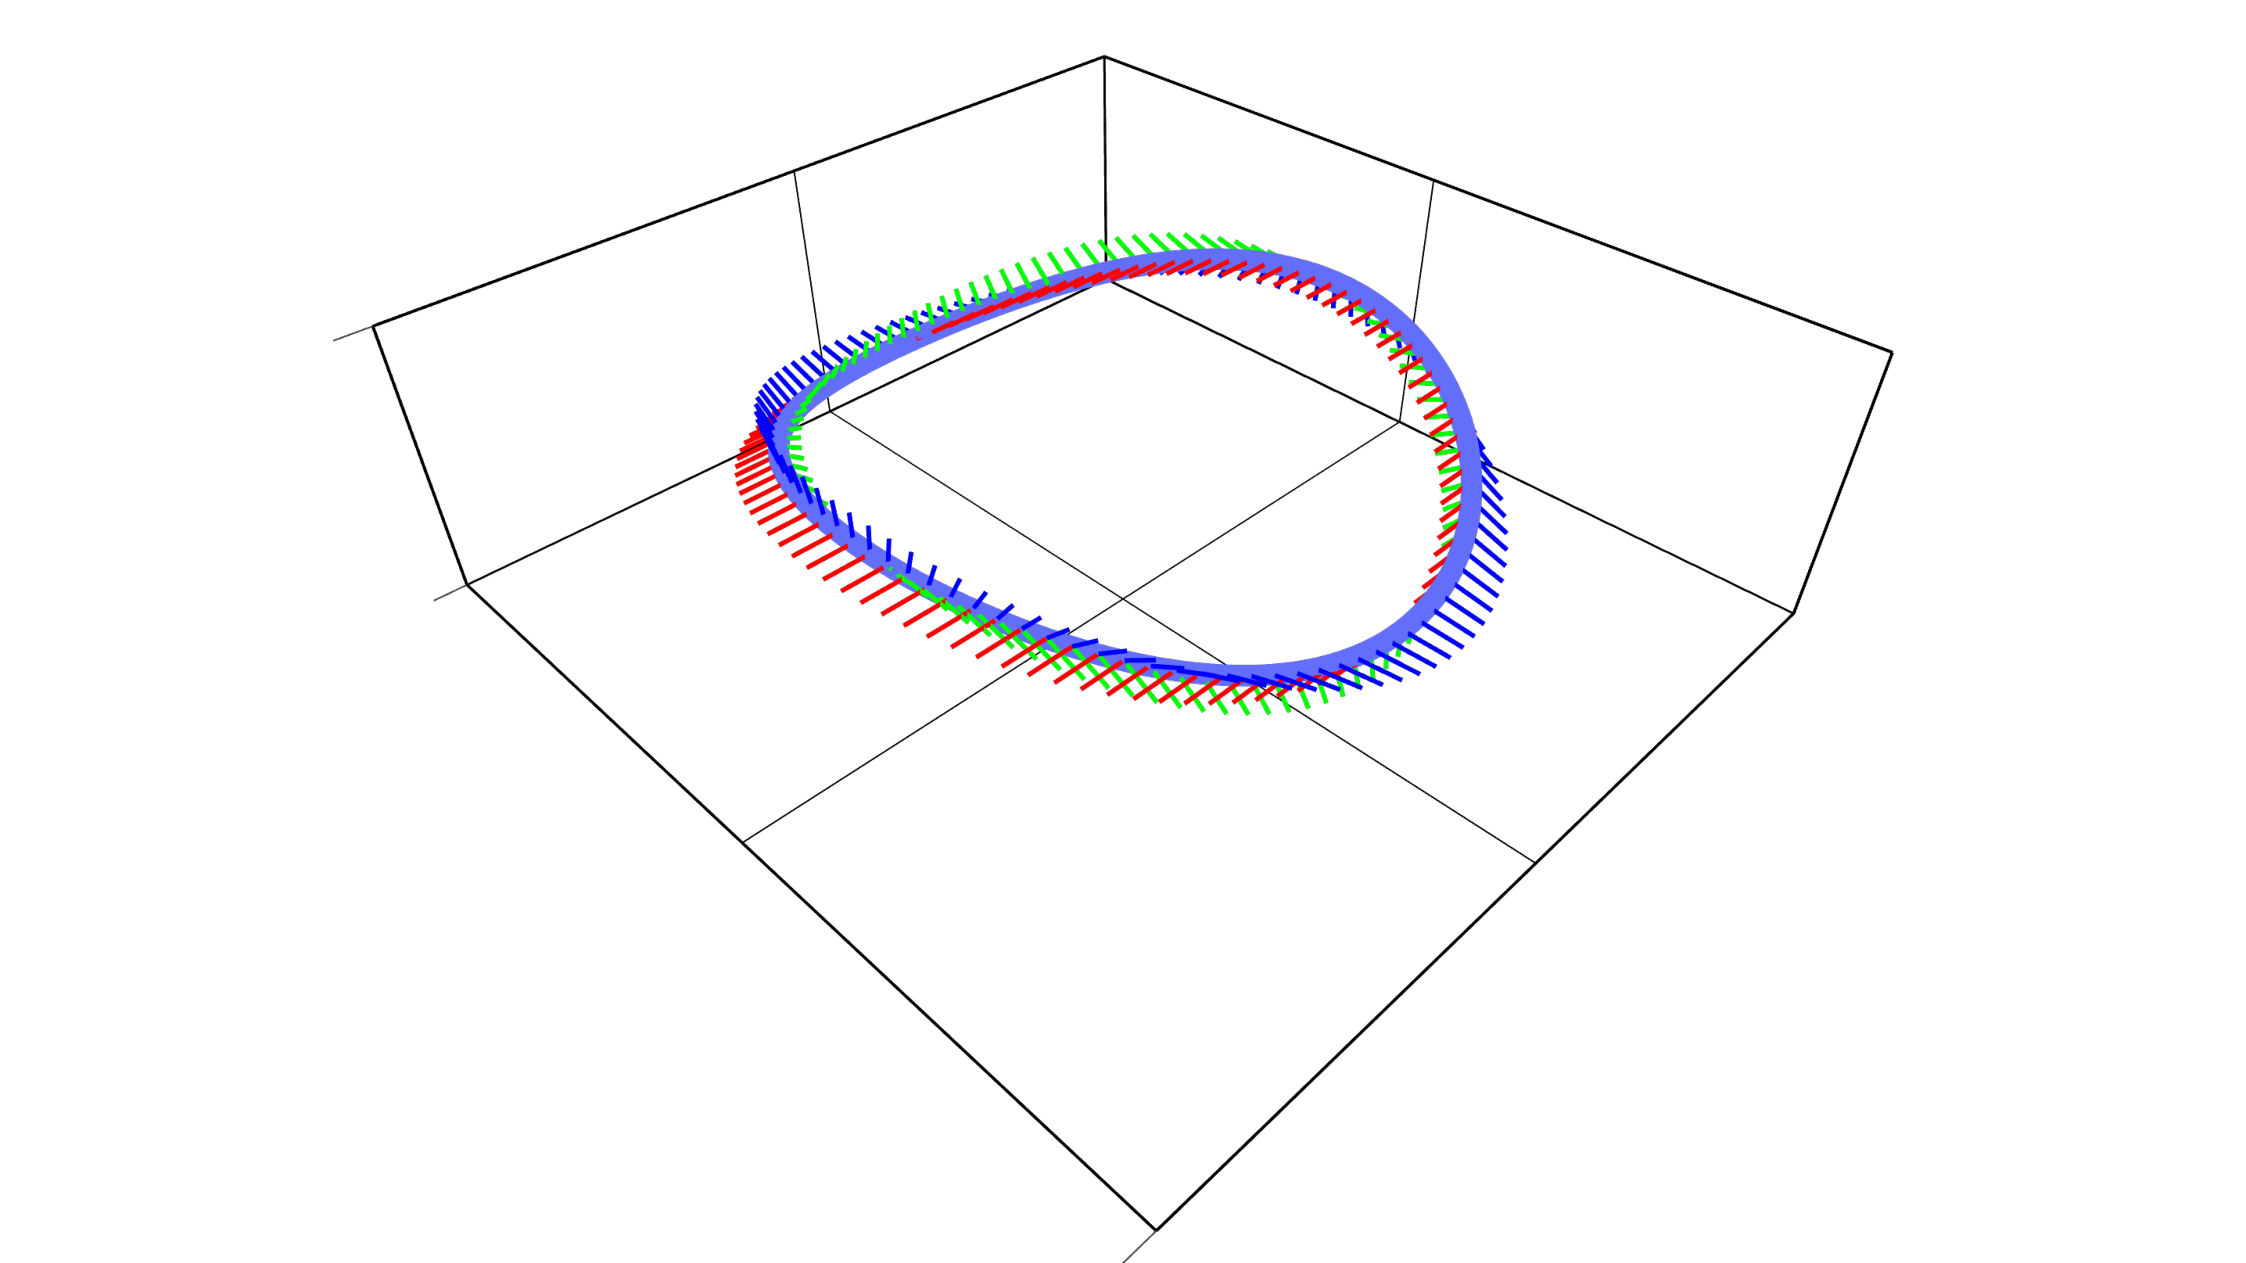
\includegraphics[width=.8\linewidth]{figures/curve_with_frames.pdf}
    \caption{Curve $\mathcal{C}$ in $\mathbb{R}^3\times\text{SO}(3)$. Orientation frames are depicted using RGB axes.}
    \label{fig:curvewithframes}
\end{figure}

The task can be achieved determining a control input $\boldsymbol{\xi}$ such that the body follows the curve $\mathcal{C}$ under a kinematic model. Although the system model was developed using the tuple representation of $\mathbb{R}^3\times\text{SO}(3)$, in this section we adopt the independent representation of $\text{ISE}(3)$, as it simplifies the control design. Note that this identification is always possible, since for any $\mathbf{H}\in\text{ISE}(3)$, we can identify $\boldsymbol{\chi}=(\mathbf{p}, \mathbf{R})$ using the following map
\begin{align}
    \begin{split}
        \mathbf{H} &\mapsto (\mathbf{B}\mathbf{H}\mathbf{c},\, \mathbf{A}\mathbf{H}\mathbf{A}^\top) \in \mathbb{R}^3\times\text{SO}(3),\\
        \mathbf{A} &= \begin{bmatrix}
            \mathbf{I}_{3\times 3} & \mathbf{0}_{3\times 4}
        \end{bmatrix}, \quad
        \mathbf{B} = \begin{bmatrix}
            \mathbf{0}_{3\times 3} & \mathbf{I}_{3\times 3} & \mathbf{0}
        \end{bmatrix}, \quad
        \mathbf{c} = \begin{bmatrix}
            \mathbf{0}^\top & 1
        \end{bmatrix}^\top.
    \end{split}
\end{align}

Now, let the system state be represented by an element $\mathbf{H}(t)\in\text{ISE}(3)$, with a generalized twist $\boldsymbol{\xi}\in\mathbb{R}^6$. Given a curve parametrization $\mathbf{H}_d(s)\in\text{ISE}(3)$, we want to compute a vector field $\Psi:\text{ISE}(3)\to\mathbb{R}^6$ such that if $\boldsymbol{\xi} = \Psi(\mathbf{H})$, the system follows the curve $\mathcal{C}$. The system can be described through the following model:
\begin{align}
% \begin{split}
    \dot{\mathbf{H}} &= \SL[\boldsymbol{\xi}]\mathbf{H}.\label{eq:first-order-system-cba}
% \end{split} 
\end{align}

In order to use our vector field methodology, we define an EE-distance function $\widehat{D}: \text{ISE}(3) \times \text{ISE}(3) \to \mathbb{R}_+$ between two elements $\mathbf{V}, \mathbf{W}$ in the group $\text{ISE}(3)$ as follows:
\begin{align}
    \widehat{D}(\mathbf{V}, \mathbf{W}) = \| \log(\mathbf{V}^{-1}\mathbf{W}) \|_F. \label{eq:cba-distance-new}
\end{align}
Note that this is exactly the same distance as defined in \cref{sec:kinematic-path-ee-dist-exp-group}, and so it possesses the same properties.
\begin{remark}
    In our original approach \citep{Pessoa2024}, we treat our system directly in $\mathbb{R}^3\times\text{SO}(3)$, and use the following distance function between two tuples:
    \begin{align}
        \widehat{D}(\mathbf{p}_1, \mathbf{R}_1, \mathbf{p}_2, \mathbf{R}_2) \triangleq \frac{1}{2}\left(\|\mathbf{p}_1 - \mathbf{p}_2\|^2 + \beta\left\|\mathbf{I} - \mathbf{R}_2^{T}\mathbf{R}_1\right\|^2_F\right). \label{eq:cba-distance}
    \end{align}
    Although \eqref{eq:cba-distance-new} and \eqref{eq:cba-distance} are not equivalent, the change in the distance function will maintain consistency with our generalization to matrix Lie groups.
    
    Note that the distance in \eqref{eq:cba-distance} is left-invariant, and although it lacks a chainability proof, we can still show that the vector field it renders has a measure zero set of singularities. This change of distance is beneficial, as it aligns with all the properties and proofs given.
\end{remark}

We will assume that the target curve $\mathcal{C}$ is twice differentiable, closed, and without self-intersections. Thus, for an element $\mathbf{H}\in\text{ISE}(3)$ and a curve parametrization $\mathbf{H}_d(s)\in\text{ISE}(3)$, the vector field has the same expression
\begin{align}
    \Psi(\mathbf{H}) = k_N(\mathbf{H})\boldsymbol{\xi}_N(\mathbf{H}) + k_T(\mathbf{H})\boldsymbol{\xi}_T(\mathbf{H}).
\end{align}
By following this vector field, the system \eqref{eq:first-order-system-cba} will converge to and follow the target curve.

\subsection{Computation of the EE-distance}\label{sec:collaborative-ee-distance-computation}
It is possible to use a simple algorithm to compute the defined EE-distance \eqref{eq:cba-distance-new}. First, note that for any elements $\mathbf{V}, \mathbf{W}\in\text{ISE}(3)$, we can write
\begin{align}
    \mathbf{V}^{-1}\mathbf{W} = \mathbf{Z} = \begin{bmatrix}
        \mathbf{R}_v^\top\mathbf{R}_w & \mathbf{0} & \mathbf{0}\\
        \mathbf{0} & \mathbf{I} & \mathbf{p}_w - \mathbf{p}_v\\
        \mathbf{0} & \mathbf{0} & 1
    \end{bmatrix} = \begin{bmatrix}
        \mathbf{Q} & \mathbf{0} & \mathbf{0}\\
        \mathbf{0} & \mathbf{I} & \mathbf{u}\\
        \mathbf{0} & \mathbf{0} & 1
    \end{bmatrix},
\end{align}
where $\mathbf{R}_v$, $\mathbf{R}_w$, $\mathbf{p}_v$, and $\mathbf{p}_w$ are the rotation matrices and positions of $\mathbf{V}$ and $\mathbf{W}$, respectively. Using Cayley-Hamilton's theorem and properties of block triangular matrices, it is possible to write
\begin{align}
    \log(\mathbf{Z}) &= \begin{bmatrix}
        \log\mathbf{Q} & \mathbf{0} & \mathbf{0}\\
        \mathbf{0} & \mathbf{0} & \mathbf{u}\\
        \mathbf{0} & \mathbf{0} & 0
    \end{bmatrix}.
\end{align}
Now, applying the Frobenius norm, we have
\begin{align}
    \|\log(\mathbf{Z})\|_F^2 &= \tr\bigl(\log(\mathbf{Z})^\top\log(\mathbf{Z})\bigr)^\frac{1}{2} = \tr\!\left(\begin{bmatrix}
        (\log\mathbf{Q})^\top\log\mathbf{Q} & \mathbf{0} & \mathbf{0}\\
        \mathbf{0} & \mathbf{0} & \mathbf{0}\\
        \mathbf{0} & \mathbf{0} & \mathbf{u}^\top\mathbf{u}
    \end{bmatrix}\right)^\frac{1}{2} \\
    &= \sqrt{\|\log\mathbf{Q}\|_F^2 + \|\mathbf{u}\|^2} = \sqrt{2\theta^2 + \|\mathbf{u}\|^2},
\end{align}
where $\theta$ is the rotation angle as in \cref{app:rodrigues-formula}. Thus, in this case the algorithm to compute the EE-distance is a simplified version of \cref{alg:dhat-se3}, as shown in \cref{alg:distance-ise3-explicit}.
\begin{algorithm}
    \caption{Computation of $\widehat{D}(\mathbf{V}, \mathbf{W})$ in $\text{ISE}(3)$}
    \label{alg:distance-ise3-explicit}
    \begin{algorithmic}[1]\label{alg:dhat-ise3}
        \Statex \textbf{Input:} Matrices $\mathbf{V}, \mathbf{W}$
        \Statex \textbf{Output:} Distance $\widehat{D}$
        % \Statex
        
        \State Compute $\mathbf{Z} \gets \mathbf{V}^{-1}\mathbf{W}$
        \State Extract $\mathbf{Q} \gets \text{rotation part of } \mathbf{Z}$ and $\mathbf{u} \gets \text{translation part of } \mathbf{Z}$

        \State $u \gets \frac{1}{2} (\tr(\mathbf{Q}) - 1)$
        \State $v \gets \frac{1}{2\sqrt{2}} \|\mathbf{Q} - \mathbf{Q}^\top\|_F$
        \State $\theta \gets \text{atan2}(v, u)$
        \State $\widehat{D} \gets \sqrt{2\theta^2 + \mathbf{u}^\top\mathbf{u}}$
    \end{algorithmic}
\end{algorithm}

% To begin, we define an error function $\widehat{D}\equiv\widehat{D}(\mathbf{p}, \mathbf{R}, \mathbf{p}_d, \mathbf{R}_d)$ that measures the discrepancy between a pose $(\mathbf{p}, \mathbf{R})$ and a desired pose $(\mathbf{p}_d, \mathbf{R}_d)$. The error function is expressed as follows
% \begin{equation}
%     \widehat{D}(\mathbf{p}, \mathbf{R}, \mathbf{p}_d, \mathbf{R}_d) \equiv \frac{1}{2}\left(\|\mathbf{p} - \mathbf{p}_d\|^2 + \beta\left\|\mathbf{I} - \mathbf{R}_d^{T}\mathbf{R}\right\|^2_F\right),\! \label{eq:errorfuncDtilde}
% \end{equation}
% where $\beta$ is a scaling parameter in squared meters utilized to maintain dimensional consistency. The Frobenius norm measures the parallelism of the rotation matrices columns, allowing parameter $\beta$ to balance position and orientation errors.

\section{Adaptive control}
In this section, we develop the adaptive control strategy to guide the manipulated object along the predefined curve $\mathcal{C}\subset \mathbb{R}^3\times \text{SO}(3)$. The goal is to provide the necessary total wrench $\boldsymbol{\tau}$ to ensure the system's velocity converges to the vector field $\Psi$, thereby enabling the object to follow the curve $\mathcal{C}$.

To develop this dynamic controller,  we modify the adaptive control strategy proposed in \cite{Culbertson2021}. In their approach, an error vector is established between the system velocity and a velocity reference, resulting in a non-autonomous system. In contrast, our method defines the velocity error $\boldsymbol{\zeta}$ with respect to the vector field, thereby establishing an autonomous system. This error vector is expressed as:
\begin{equation}
    \boldsymbol{\zeta} = \dot{\boldsymbol{\chi}} - \Psi. \label{eq:errorvector-s}
\end{equation}
If the dynamic controller guarantees that $\boldsymbol{\zeta}$ goes to zero, the system follows the kinematic model \eqref{eq:first-order-system-cba}, with the vector field $\Psi$ acting as its input. Therefore, as shown in \cref{ch:vector_field}, we anticipate that the system will exhibit the desired behavior. To develop the adaptive control strategy, we first define our reference model.

Given that the system is overactuated (meaning multiple sets of control inputs $\boldsymbol{\tau}_i$ produce identical object dynamics), each agent can contribute a portion of the control effort. Thus, we define a set of $N$ positive constants $\alpha_i$, ensuring $\sum_{i=1}^N\alpha_i=1$. Furthermore, analogously to the Euler-Lagrange formulation, the reference model can be linearly parametrized. Thus, the reference model can be expressed as 
\begin{equation}
    \alpha _i \left(\mathbf {M}(\boldsymbol{\chi})\dot{\Psi} + \mathbf {C}(\boldsymbol{\chi},\dot{\boldsymbol{\chi}})\Psi + \mathbf {g} \right) = \mathbf{Y}_o(\boldsymbol{\chi}, \dot{\boldsymbol{\chi}}, \Psi, \dot{\Psi})\mathbf{o}_i, \label{eq:ref-model-linear-parametrization}
\end{equation}
% Furthermore, exploiting the linearity in the parameters within the equations of motion \citep{spong2020robot}, we can represent the object's dynamics using a regressor matrix $\mathbf{Y}_o$ and a parameter vector $\mathbf{o}_i$. Here, $\mathbf{o}_i = \alpha_i\mathbf{o}$ denotes a vector of the object's physical parameters, $\mathbf{o}$, such as mass or moments of inertia, scaled by $\alpha_i$:
% Analogously to the Euler-Lagrange formulation, the reference model can be linearly parametrized as
% \begin{align}
%     \boldsymbol{\tau}_i &= \mathbf{Y}_o(\boldsymbol{\chi}, \dot{\boldsymbol{\chi}}, \boldsymbol{\Psi}, \dot{\boldsymbol{\Psi}})\mathbf{o}_i, \label{eq:ref-model-linear-parametrization}
% \end{align}
where $\mathbf{Y}_o$ is the regressor matrix given by
\begin{align}
    \mathbf{Y}_o &= \begin{bmatrix}
        \ddot{\mathbf{p}}_d & -\SL[\dot{\boldsymbol{\omega}}_d]\mathbf{R}-\SL[\boldsymbol{\omega}]\SL[\boldsymbol{\omega}_d]\mathbf{R} & \mathbf{0}\\
        \mathbf{0} & \SL[\ddot{\mathbf{p}}_d]\mathbf{R} + \SL[\boldsymbol{\omega}]\SL[\dot{\mathbf{p}}_d]\mathbf{R} - \SL[\boldsymbol{\omega}_d]\SL[\dot{\mathbf{p}}]\mathbf{R} & \mathbf{R}\mathcal{J}\bigl(\mathbf{R}\dot{\boldsymbol{\omega}}_d\bigr) + \SL[\boldsymbol{\omega}]\mathbf{R}\mathcal{J}\bigl(\mathbf{R}^\top\boldsymbol{\omega}_d\bigr)
    \end{bmatrix},
\end{align}
where $\mathcal{J}:\mathbb{R}^3\to\mathbb{R}^{3\times6}$ is the following map
\begin{align}
    \mathcal{J}\bigl([a_1\ a_2\ a_3]^\top\bigr)=\begin{bmatrix}
        a_1 & a_2 & a_3 & 0 & 0 & 0 \\
        0 & a_1 & 0 & a_2 & a_3 & 0 \\
        0 & 0 & a_1 & 0 & a_2 & a_3
    \end{bmatrix}.
\end{align}
The term $\mathbf{o}_i$ is the parameter vector given by
\begin{align}   
    \mathbf{o}_i &= \alpha_i\begin{bmatrix}
        m & m\mathbf{r}_p & \{\mathbb{I}_p\}_{11} & \{\mathbb{I}_p\}_{12} & \{\mathbb{I}_p\}_{22} & \{\mathbb{I}_p\}_{23} & \{\mathbb{I}_p\}_{33}
    \end{bmatrix}^\top,
\end{align}
where $\{\mathbb{I}_p\}_{ij}$ are the elements of the inertia matrix $\mathbb{I}_p^\mathfrak{B}$ at the $i^{th}$ row and $j^{th}$ column. Note that, since the inertia tensor is symmetric, we only need to consider the upper triangular part of the matrix. Also, note that the sum $\sum_{i=1}^N\mathbf{Y}_o\mathbf{o}_i=\mathbf{Y}_o\mathbf{o}$ results in the total wrench $\boldsymbol{\tau}$ applied to the object. Moreover, since the agents estimate the scaled vector $\mathbf{o}_i$, the constants $\alpha_i$ need not be known a priori.

Next, we propose the following control law
\begin{equation}
    \boldsymbol{\tau}_i = \boldsymbol{\Lambda}(\boldsymbol{\chi}, \hat{\mathbf{r}}_i)^{-1}\boldsymbol{\eta}_i,\label{eq:controlLawTaui}
\end{equation}
where $\hat{\mathbf{r}}_i$ represents the estimate of the $i^{th}$ agent's displacement with respect to the measurement point, and
\begin{equation}
    \boldsymbol{\eta}_i = \mathbf{Y}_o\hat{\mathbf{o}}_i - \mathbf{K}_D\boldsymbol{\zeta}, \label{eq:controlLawEtai}
\end{equation}
where $\mathbf{K}_D$ is a positive definite matrix, and $\hat{\mathbf{o}}_i$ is the $i^{th}$ agent's estimate of the object's parameters. 

% It is essential to note that:
% \begin{equation}
%     \mathbf{G}_i\mathbf{G}(\hat{\mathbf{r}}_i)^{-1} = \mathbf{I} - \mathbf{G}(\widetilde{\mathbf{r}}_i), \label{eq:relationGiGiInvtoProof}
% \end{equation}
% where $\widetilde{\mathbf{r}}_i = \hat{\mathbf{r}}_i - \mathbf{r}_i$.

If we let $\widetilde{\mathbf{r}}_i = \hat{\mathbf{r}}_i - \mathbf{r}_i$, we can achieve the following linear parametrization:
\begin{equation}
    -\boldsymbol{\Lambda}(\boldsymbol{\chi}, \widetilde{\mathbf{r}}_i)\boldsymbol{\eta}_i = \mathbf{Y}_r\left(\boldsymbol{\eta}_i, \boldsymbol{\chi}\right)\widetilde{\mathbf{r}}_i. \label{eq:linearParametrizationYrforEta}
\end{equation}
With this parametrization and the other expressions, we propose the following adaptation laws:
\begin{align}
    \dot{\hat{\mathbf{o}}}_i &= -\boldsymbol{\Gamma}_o\mathbf{Y}^\top_o\left(\boldsymbol{\chi},\dot{\boldsymbol{\chi}},\Psi, \dot{\Psi}\right)\boldsymbol{\zeta},  \label{eq:adaptiveOhat}\\
    \dot{\hat{\mathbf{r}}}_i &= -\boldsymbol{\Gamma}_r\mathbf{Y}^\top_r\left(\boldsymbol{\eta}_i, \boldsymbol{\chi}\right)\boldsymbol{\zeta},  \label{eq:adaptiveRhat}
\end{align}
where $\boldsymbol{\Gamma}_o$ and $\boldsymbol{\Gamma}_r$ are definite positive matrices corresponding to the adaptation gains. With the proposed control law \eqref{eq:controlLawTaui} and adaptation laws \eqref{eq:adaptiveOhat} and \eqref{eq:adaptiveRhat}, we can guarantee that the system follows the curve $\mathcal{C}$ as proven in the following theorem.
\begin{theorem}
    Under the adaptive control laws \eqref{eq:controlLawTaui} and \eqref{eq:controlLawEtai}, and adaptation laws \eqref{eq:adaptiveOhat} and \eqref{eq:adaptiveRhat}, the system converges to and follows the curve $\mathcal{C}$.
\end{theorem}
\begin{proof}
    Consider the following Lyapunov function candidate
    \begin{equation}
        V = \frac{1}{2}\left( \boldsymbol{\zeta}^\top \mathbf {M} \boldsymbol{\zeta} + \sum _{i=1}^{N} \left(\widetilde{\mathbf{o}}_i^\top \boldsymbol{\Gamma }_o^{-1}\widetilde{\mathbf{o}}_i + \widetilde{\mathbf{r}}_i^\top \boldsymbol{\Gamma }_r^{-1} \widetilde{\mathbf{r}}_i \right)\right),
    \end{equation}
    where $\widetilde{\mathbf {o}}_i = \hat{\mathbf{o}}_i - \mathbf{o}_i$ represents the parameter estimation error for the $i^{th}$ agent.

    Since the true parameters do not vary in time, i.e. $\dot{\widetilde{\mathbf {o}}}_i = \dot{\hat{\mathbf{o}}}_i$ and $\dot{\widetilde{\mathbf {r}}}_i = \dot{\hat{\mathbf{r}}}_i$, the time derivative of the Lyapunov candidate yields
    \begin{equation}
        \dot{V} = \boldsymbol{\zeta}^\top \mathbf{M} \dot{\boldsymbol{\zeta}} + \frac{1}{2} \boldsymbol{\zeta}^\top \dot{\mathbf{M}} \boldsymbol{\zeta} + \sum\limits_{i=1}^{N}\left( \widetilde{\mathbf{o}}_i^\top \boldsymbol{\Gamma}_o^{-1} \dot{\hat{\mathbf{o}}}_i + \widetilde{\mathbf{r}}_i^\top \boldsymbol{\Gamma}_r^{-1}\dot{\hat{\mathbf{r}}}_i\right).
        \label{eq:adaptive-lyapunov-derivative}
    \end{equation}
    Using the fact that $\dot{\boldsymbol{\zeta}} = \ddot{\boldsymbol{\chi}} - \dot{\Psi}$ and $\dot{\boldsymbol{\chi}} = \boldsymbol{\zeta} + \Psi$, along with the system dynamics equation \eqref{eq:tau} and expression \eqref{eq:tauNtauIrelation}, and \eqref{eq:ref-model-linear-parametrization}, we can express the first term as
    \begin{align} 
    \begin{split}
        \boldsymbol{\zeta}^\top \mathbf {M} \dot{\boldsymbol{\zeta}} &= \boldsymbol{\zeta}^\top\mathbf{M}\bigl(\ddot{\boldsymbol{\chi}} - \dot{\Psi}\bigr)
        = \boldsymbol{\zeta}^\top\bigl(\boldsymbol{\tau} - \mathbf{C}\dot{\boldsymbol{\chi}} - \mathbf{g} - \mathbf{M}\dot{\Psi}\bigr)\\
        &= \boldsymbol{\zeta}^\top\Biggl(\biggl(\sum_{i=1}^N\boldsymbol{\Lambda}(\boldsymbol{\chi}, \mathbf{r}_i)\boldsymbol{\tau}_i\biggr) -\mathbf{C}\Psi - \mathbf{C}\boldsymbol{\zeta} - \mathbf{g} - \biggl(-\mathbf{C}\Psi-\mathbf{g}+\sum_{i=1}^N\mathbf{Y}_o\mathbf{o}_i\biggr)\Biggr)\\
        &= \boldsymbol{\zeta}^\top\Biggl( - \mathbf{C}\boldsymbol{\zeta}+\sum_{i=1}^N\boldsymbol{\Lambda}(\boldsymbol{\chi}, \mathbf{r}_i)\boldsymbol{\tau}_i - \mathbf{Y}_o\mathbf{o}_i \Biggr).
    \end{split} \label{eq:partial-term-of-adaptive1}
    \end{align} 
    Now, using equations \eqref{eq:controlLawTaui}, \eqref{eq:controlLawEtai} and \eqref{eq:linearParametrizationYrforEta}, the first term in \eqref{eq:partial-term-of-adaptive1} can be rewritten as
    \begin{align}
        \boldsymbol{\zeta}^\top \mathbf {M} \dot{\boldsymbol{\zeta}} &= \boldsymbol{\zeta}^\top\Biggl( - \mathbf{C}\boldsymbol{\zeta} + \sum_{i=1}^N\boldsymbol{\Lambda}(\boldsymbol{\chi}, \mathbf{r}_i)\boldsymbol{\Lambda}(\boldsymbol{\chi}, \hat{\mathbf{r}}_i)^{-1}\boldsymbol{\eta}_i - \mathbf{Y}_o\mathbf{o}_i\Biggr)\\
        &= \boldsymbol{\zeta}^\top\Biggl(- \mathbf{C}\boldsymbol{\zeta}+\sum_{i=1}^N(\mathbf{I}-\boldsymbol{\Lambda}(\boldsymbol{\chi}, \widetilde{\mathbf{r}}_i))\boldsymbol{\eta}_i - \mathbf{Y}_o\mathbf{o}_i \Biggr)\\
        &= \boldsymbol{\zeta}^\top\Biggl(- \mathbf{C}\boldsymbol{\zeta} + \sum_{i=1}^N \biggl( \mathbf{Y}_o\hat{\mathbf{o}}_i + \mathbf{Y}_r\widetilde{\mathbf{r}}_i - \mathbf{Y}_o\mathbf{o}_i- \mathbf{K}_D\boldsymbol{\zeta}\biggr) \Biggr)\\
        &= \boldsymbol{\zeta}^\top\Biggl(- \mathbf{C}\boldsymbol{\zeta} + \sum_{i=1}^N\biggl( \mathbf{Y}_o\widetilde{\mathbf{o}}_i + \mathbf{Y}_r\widetilde{\mathbf{r}}_i - \mathbf{K}_D\boldsymbol{\zeta}\biggr) \Biggr). \label{eq:partial-term-of-adaptive2}
    \end{align}

    Finally, substituting \eqref{eq:partial-term-of-adaptive2} into \eqref{eq:adaptive-lyapunov-derivative} renders the following result
    \begin{align}
    % \begin{split}
        \dot{V} &= \frac{1}{2}\boldsymbol{\zeta}^\top \bigl(\dot{\mathbf{M}}- 2\mathbf{C}\bigr) \boldsymbol{\zeta} + \sum\limits_{i=1}^{N} \left(\widetilde{\mathbf{o}}_i^\top \boldsymbol{\Gamma}_o^{-1} \dot{\hat{\mathbf{o}}}_i + \widetilde{\mathbf{r}}_i^\top \boldsymbol{\Gamma}_r^{-1}\dot{\hat{\mathbf{r}}}_i + \boldsymbol{\zeta}^\top\bigl(\mathbf{Y}_o\widetilde{\mathbf{o}}_i + \mathbf{Y}_r\widetilde{\mathbf{r}}_i - \mathbf{K}_D\boldsymbol{\zeta} \bigr)\right).
        % \end{split}
    \end{align}
    Substituting adaptation laws \eqref{eq:adaptiveOhat} and \eqref{eq:adaptiveRhat}, and using the fact that $\dot{\mathbf{M}} - 2\mathbf{C}$ is skew-symmetric, we have
    \begin{align}
        \dot{V} &= \sum\limits_{i=1}^{N} -\widetilde{\mathbf{o}}_i^\top \mathbf{Y}^\top_o\boldsymbol{\zeta}  - \widetilde{\mathbf{r}}_i^\top\mathbf{Y}^\top_r\boldsymbol{\zeta} + \boldsymbol{\zeta}^\top\mathbf{Y}_o\widetilde{\mathbf{o}}_i + \boldsymbol{\zeta}^\top\mathbf{Y}_r\widetilde{\mathbf{r}}_i - \boldsymbol{\zeta}^\top\mathbf{K}_D\boldsymbol{\zeta}.
    \end{align}
    Since all terms are scalars, we can transpose the first two terms and achieve the following result
    \begin{align}
        \dot{V} = \sum\limits_{i=1}^{N}-\boldsymbol{\zeta}^\top\mathbf{K}_D\boldsymbol{\zeta} = -N\boldsymbol{\zeta}^\top\mathbf{K}_D\boldsymbol{\zeta} \le 0.
    \end{align}
    Since $N$ is positive and $\mathbf{K}_D$ is definite positive, $\boldsymbol{\zeta}$ converges to zero as $t$ goes to $\infty$. This implies that the velocity error is zero and the system behaves as the kinematic model \eqref{eq:first-order-system-cba}. Thus we can invoke \cref{thm:convergence-vector-field} to conclude that the system converges to and follows the curve $\mathcal{C}$.
\end{proof}

The connection of both controllers is shown in the block diagram of \cref{fig:collaborative-full-diagram}.
\begin{figure}[ht]
    \centering
    \resizebox{\textwidth}{!}{%
    \begin{tikzpicture}[
        block/.style={draw, rectangle, minimum height=1.2cm, minimum width=2.4cm, align=center},
        arrow/.style={->, >=stealth, thick},
        label/.style={font=\small},
        sumblock/.style={draw, circle, minimum size=0.8cm}
    ]
    
    % Nodes
    \node[block] (kinematic) {Vector Field};
    \node[block, right=2cm of kinematic] (refmodel) {Reference\\Model};
    % \node[block, right=2cm of kinematic] (plant) {Plant \\ $P(\theta)\to P_c(\theta_c)$};
    \node[block, right=1cm of refmodel] (control) {Dynamic\\Controller};
    \node[block, above=0.75cm of control] (estimation) {Estimation\\of $\mathbf{o}_i, \mathbf{r}_i$};
    \node[block, above=1cm of estimation, xshift=-1cm] (mapping) {Mapping\\$\mathbb{R}^3\times\text{SO}(3)\to\text{ISE}(3)$};
    \node[block, right=1cm of control] (plant) {System};
    \node[left=0.75cm of kinematic,yshift=-0.25cm] (input) {Curve $\mathcal{C}$};
    \node[sumblock, left=2cm of estimation, yshift=-0.25cm] (sum) {};
    \node at ([xshift=0.2cm]sum.west) {\(+\)};
    \node at ([yshift=-0.2cm]sum.north) {\(-\)};
    \node[right=1.5cm of plant] (output) {$\boldsymbol{\chi}$};
    
    % Arrows between blocks
    \draw[arrow] (input) -- ($(kinematic.west)+(0,-0.25cm)$);
    \draw[arrow] (plant.east) -- (output);
    % Ends in refmodel
    \draw[arrow] (kinematic) -- node[below, label] {$\Psi, \dot{\Psi}$} (refmodel);
    \draw[arrow] ($(plant.east)+(0.75, 0)$) |- ($(refmodel.south)+(0,-1)$) -| node[right, label,yshift=0.25cm] {$\boldsymbol{\chi}, \dot{\boldsymbol{\chi}}$} (refmodel.south);
    % Ends in System
    \draw[arrow] (control) -- node[above, label] {$\boldsymbol{\tau}_i$} (plant);
    % Ends in mapping
    \draw[arrow] ($(plant.east)+(0.75,0)$) |- (mapping.east) node[right, yshift=0.25cm, label] {$\boldsymbol{\chi}\in\mathbb{R}^3\times\text{SO}(3)$};
    % Ends in Estimation
    \draw[arrow] (sum.east) -- node[below,label] {$\boldsymbol{\zeta}$} ($(estimation.west)+(0,-0.25)$);
    \draw[arrow] ($(plant.east)+(0.75,0)$) |- (estimation.east) node[right, label, yshift=0.25cm] {$\boldsymbol{\chi}, \dot{\boldsymbol{\chi}}$};
    \draw[arrow] ($(refmodel.east)+(0.5,0)$) |- ($(estimation.west)+(0,0.25)$);
    % Ends in Vector Field
    \draw[arrow] (mapping.west) node[left, yshift=0.25cm, label] {$\mathbf{H}\in\text{ISE}(3)$} -| ($(kinematic.west)+(-0.75,1)$) |- ($(kinematic.west)+(0,0.25)$);
    % Ends in Control
    \draw[arrow] (estimation.south) -- node[right, label] {$\widehat{\mathbf{o}}_i, \widehat{\mathbf{r}}_i$} (control.north);
    \draw[arrow] (refmodel.east) -- node[below, label] {$\mathbf{Y}_o$} (control.west);
    \draw[arrow] ($(estimation.west)+(-0.25,-0.25)$) |- ($(control.west)+(0,0.25)$);
    \draw[arrow] ($(plant.east)+(0.75, 0)$) |- ($(control.south)+(0,-0.5)$) -| node[right, label,yshift=0.25cm] {$\boldsymbol{\chi}$} (control.south);
    % Ends in summation block
    \draw[arrow] ($(kinematic.east)+(1,0)$) |- node[left, label] {$\Psi$} (sum.west);
    \draw[arrow] ($(plant.east)+(0.75,0)$) |- ($(sum.north)+(0,1)$) -| node[left, label] {$\dot{\boldsymbol{\chi}}$} (sum.north);
    \end{tikzpicture}%
    }
    \caption{Block diagram of the collaborative manipulation control framework.}
    \label{fig:collaborative-full-diagram}
\end{figure}